\newpage

\chapter{Výsledky}

\section{Trénovanie}

V tréningu sa snažíme predpovedať, či v používateľskom sedení dôjde k nákupu jedného alebo viacerých produktov. Na výstupe siete teda existujú dve triedy. Vygenerujeme pravdepodobnosť, s akou patrí sedenie do konkrétnej triedy. Triedu s vyššou pravdepodobnosťou následne prehlasujeme za výsledok. \newline
Trénovanie prebiehalo za použitia optimalizačnej stratégie ADAM. Počiatočná rýchlosť učenia je 0.001. Počet neurónov skrytej vrstvy je 128.\newline
Pracujeme s podmnožinou o veľkosti 100 tisíc klikov, z ktorej je vygenerovaných 20 tisíc vstupných vektorov pre tréningovú množinu. Validačná a testovacia množina obsahujú 2,6 tisíc vektorov, tj. 10 \% datasetu pre každú. Po vyvážení tried prebieha učenie na vzorke 18 tisíc vstupných vektorov pre triedu nákupných aj nenákupných sedení. Spolu je teda sieť učená na datasete 37 tisíc vzoriek. Vzorky sú pred vstupom zamiešané a rozdelené do úsekov. Po každom úseku je evaluovaná sieť voči validačnej množine.\newline
Tréning je zastavovaný, keď validačná množina prestáva zaznamenávať zlepšovanie oproti predchádzajúcej epoche. Keďže je štatisticky možné aby sa objavilo jedno zhoršenie počas tréningu, sieť je zastavovaná ak na validačnej množine nedojde k zlepšeniu väčšiemu ako 0.25 \% 3x po sebe. 

\section{Testovanie}
\label{testing}

Popri samotnej validačnej množine sú vyhodnocované aj metriky tried klasifikácie. V tabuľkách je možné sledovať príklad z validačnej a testovacej vzorky po učení.

\parbox{.45\linewidth}{
\begin{tabular}{||c||c|c|} 
	\hline
	VALID & TRUE & FALSE \\ [0.5ex] 
	\hline\hline
	POSITIVE & 146 &  626 \\ 
	\hline
	NEGATIVE & 1797 & 36 \\
	\hline
\end{tabular}
}
\parbox{.45\linewidth}{
\begin{tabular}{||c||c|c|} 
	\hline
	TEST & TRUE & FALSE \\ [0.5ex] 
	\hline\hline
	POSITIVE & 129 &  609 \\ 
	\hline
	NEGATIVE & 1775 & 50 \\
	\hline
\end{tabular}
}
\newline

Na obrázku ~\ref{fig:validate} je možné sledovať správanie učenia neurónovej siete. Dochádza k rýchlemu zlepšeniu a následne oscilácií okolo optima, pričom sieť je zastavená keď nedochádza k priemernému zlepšeniu. Ako dôkaz nepreúčania slúži testovacia množina, ktorá dosahuje rovnaké výsledky ako validačná. Konečný výsledok pre validačnú a testovaciu množinu sa opakovane a stabilne pohybuje v rozmedzí \textbf{74-75\%} úspešnosti klasifikácie používateľského sedenia.

\begin{figure}[H]
	\begin{center}
		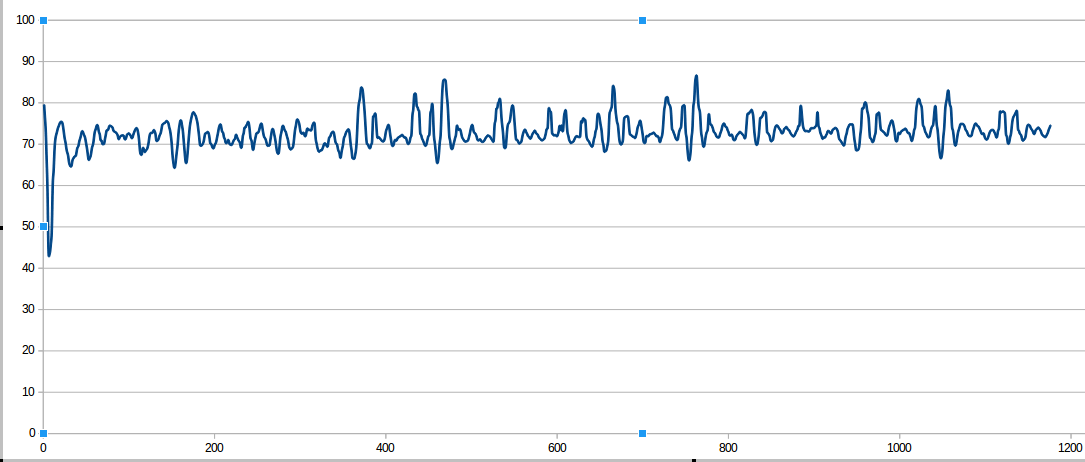
\includegraphics[scale=0.40]{validate}\end{center}
	\caption[validate]{Priebeh učenia na validačnej množine}
	\label{fig:validate}
\end{figure}

